\documentclass[paper=letter, fontsize=12pt]{article}

\usepackage{amsmath,amsfonts,amsthm, amssymb} % Math packages
\usepackage{stmaryrd}
\usepackage[shortlabels]{enumitem}
\usepackage[pdftex]{graphicx}
\usepackage{booktabs}
\usepackage{placeins}
\usepackage{algpseudocode}
\usepackage[margin=1in]{geometry}
\usepackage{listings}
\usepackage{mdframed}
\usepackage{tcolorbox}
\usepackage{float}
\usepackage{subcaption}
\usepackage{url}
\usepackage{hyperref}

\usepackage{mathtools}
\DeclarePairedDelimiterX{\norm}[1]{\lVert}{\rVert}{#1}
\DeclarePairedDelimiterX{\abs}[1]{\lvert}{\rvert}{#1}
\DeclareMathOperator*{\argmin}{arg\,min}
\DeclareMathOperator{\spn}{span}
\DeclareMathOperator{\rct}{rect}
\DeclareMathOperator{\support}{support}
\DeclareSymbolFont{matha}{OML}{txmi}{m}{it}% txfonts
\DeclareMathSymbol{\varv}{\mathord}{matha}{118}
\DeclareMathOperator{\E}{\mathbb{E}}
\DeclareMathOperator{\Tr}{Tr}

\newcommand{\ceil}[1]{\lceil #1 \rceil}
\newcommand{\floor}[1]{\lfloor #1 \rfloor}
\newcommand{\Lapl}{\mathcal{L}}
\newcommand{\reals}{\mathbb{R}}
\newcommand{\complexes}{\mathbb{C}}
\newcommand{\ints}{\mathbb{Z}}
\newcommand{\innerp}[2]{\langle #1, #2 \rangle}
\newcommand{\vecii}[2]{\begin{bmatrix} #1 \\ #2 \end{bmatrix}}
\newcommand{\veciii}[3]{\begin{bmatrix} #1 \\ #2 \\ #3 \end{bmatrix}}
\newcommand{\rect}[1]{\rct \left( #1 \right)}
\newcommand{\pw}[1]{\begin{cases} #1 \end{cases}}
\newcommand{\Mod}[1]{\ \text{mod}\ #1}
\newcommand{\sumN}{\sum\limits_{n=0}^{N-1}}
\newcommand{\sumK}{\sum\limits_{k=0}^{N-1}}
\newcommand\given[1][]{\:#1\vert\:}

\graphicspath{{img/}}

\title{CS 543 - Progress Report}
\author{
        Dario Aranguiz \\
        Cu-Khoi-Nguyen Mac
        }
\date{\today}


%%% Begin document
\begin{document}
\maketitle
% \pagebreak

\section{Updated statement of the project definition and goals}

\section{Current member roles and collaboration strategies}

\section{Proposed approach}

\section{Data}

\begin{figure}[htbp]
	\centering
	\begin{subfigure}[b]{0.32\linewidth}
		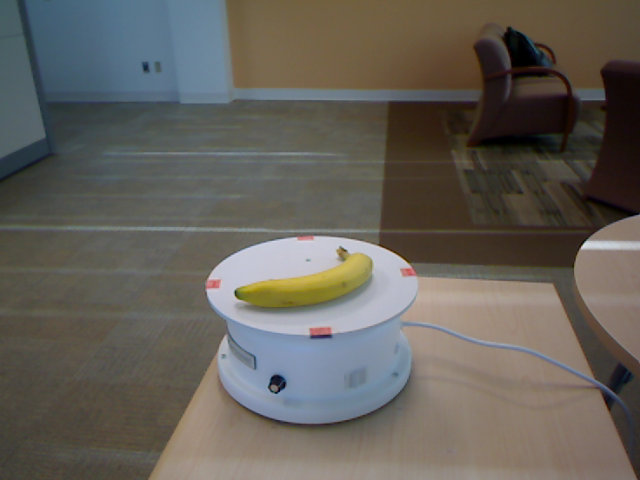
\includegraphics[width=\textwidth]{banana_1_1_1}
		\caption{Color image}
	\end{subfigure}
	\begin{subfigure}[b]{0.32\linewidth}
		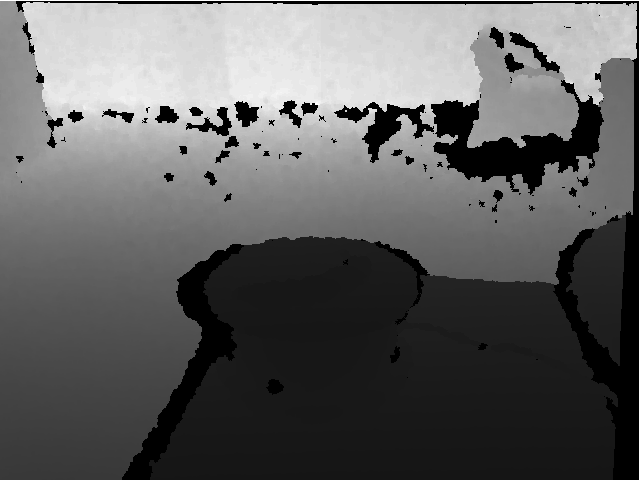
\includegraphics[width=\textwidth]{banana_1_1_1_depth}
		\caption{Depth image}
	\end{subfigure}
	\begin{subfigure}[b]{0.32\linewidth}
		
\includegraphics[width=\textwidth]{banana_1_1_1_mask}
		\caption{Mask}
	\end{subfigure}
	
	\caption{A banana sample of Washington's RGB-D object dataset.}
	\label{fig:banana}
\end{figure}

sub-dataset

\section{Initial results}

\subsection{Data preprocessing}
\begin{figure}[htbp]
	\centering
	\begin{subfigure}[b]{0.32\linewidth}
		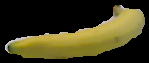
\includegraphics[width=\textwidth]{banana_1_1_1_crop}
		\caption{Color image}
	\end{subfigure}
	\begin{subfigure}[b]{0.32\linewidth}
		
\includegraphics[width=\textwidth]{banana_1_1_1_depth_crop}
		\caption{Depth image}
	\end{subfigure}
	\caption{Cropping banana sample after applying mask.}
	\label{fig:banana_crop}
\end{figure}

\begin{figure}[htbp]
	\centering
	\begin{subfigure}[b]{0.32\linewidth}
		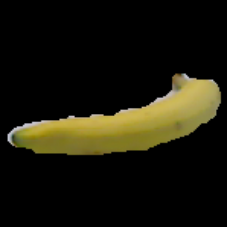
\includegraphics[width=\textwidth]{banana_1_1_1_resize}
		\caption{Color image}
	\end{subfigure}
	\begin{subfigure}[b]{0.32\linewidth}
		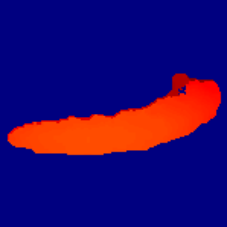
\includegraphics[width=\textwidth]{banana_1_1_1_depth_resize}
		\caption{Depth image (after colorizing)}
	\end{subfigure}
	\caption{Rescaling banana sample to 227x227 by replicating the longer side.}
	\label{fig:banana_resize}
\end{figure}

\subsection{Model architecture}
\begin{figure}[htbp]
	\centering
	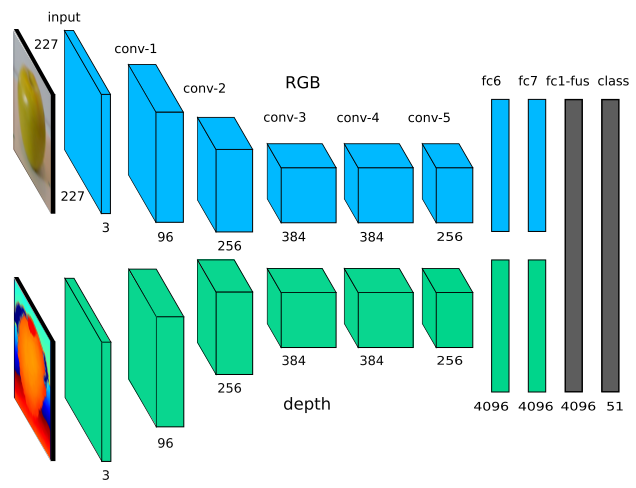
\includegraphics[width=.7\textwidth]{architecture}
	\caption{Model architecture proposed by Eitel et al. \cite{Eitel2015}.}
	\label{fig:architecture_eitel}
\end{figure}

\begin{figure}[htbp]
\centering
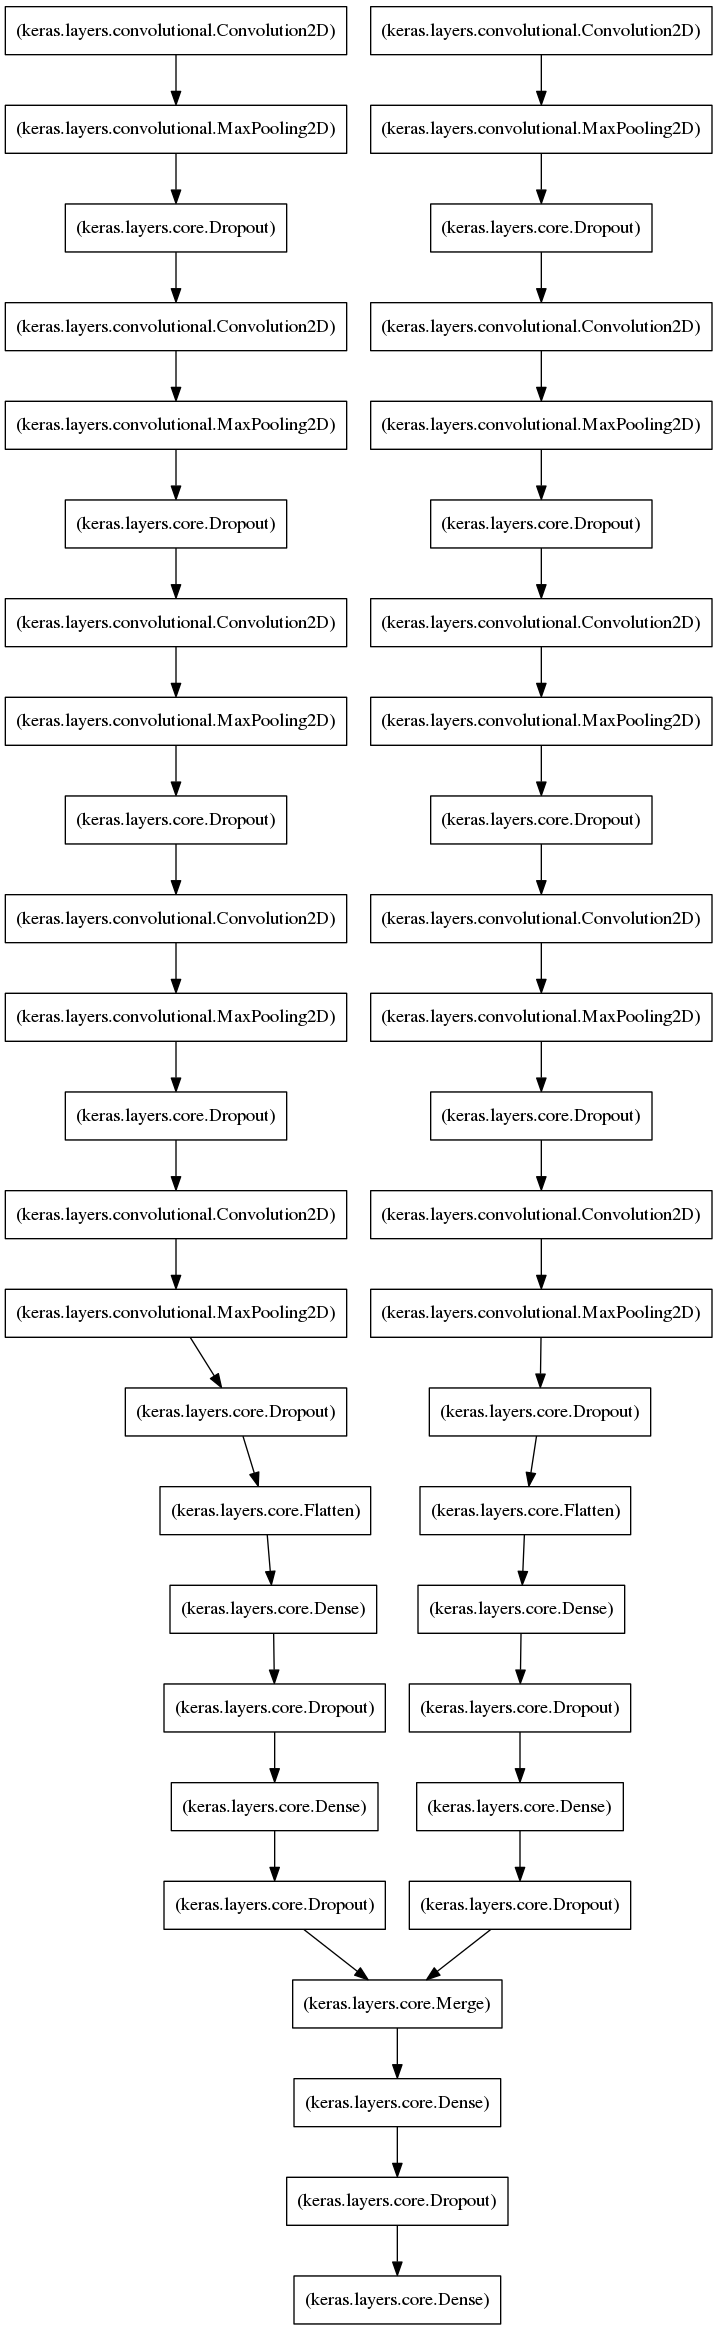
\includegraphics[width=.42\textwidth]{fusion_model}
\caption{Fusion model with RGB and depth streams.}
\label{fig:fusion_model}
\end{figure}

\section{Current reservations and questions}
(if any)

\bibliographystyle{abbrv}
\bibliography{mybib}


%%% End document
\end{document}